\documentclass[a4paper, 10pt, final, garamond]{book}
\usepackage{cours-preambule}
\graphicspath{{./figures/}}
\addto\captionsfrench{\renewcommand{\figurename}{Fig.}}

\makeatletter
\renewcommand{\@chapapp}{Contr\^ole de connaissances}
\makeatother

% \toggletrue{student}
% \toggletrue{corrige}
\renewcommand{\mycol}{black}
% \renewcommand{\mycol}{gray}

\begin{document}
\setcounter{chapter}{1}

\settype{enon}
\settype{solu}

\chapter{Dispositifs optiques\ifstudent{~(15')}}

\begin{enumerate}[label=\sqenumi, leftmargin=10pt]
	\item[n]{6} %
	Démontrer la relation de conjugaison de \textsc{Newton}. Un schéma
	est attendu.
	\smallbreak
	\begin{isd}[righthand ratio=.3]
		\psw{%
			On utilise le théorème de \textsc{Thalès} dans les triangles F$'$OH et
			F$'$A$'$B$'$, en remarquant que $\obarr{OH} = \AB$ \pt{1}, et les
			triangles FAB et FOH' pour avoir
			\begin{gather*}
				\frac{\obarr{A'B'}}{\obarr{OH}} = \frac{\ABp}{\AB} \stm{=}
				\frac{\obarr{F'A'}}{\obarr{F'O}}
				\qqet
				\frac{\obarr{OH'}}{\obarr{AB}} = \frac{\ABp}{\AB} \stm{=}
				\frac{\obarr{FO}}{\obarr{FA}}
				% \\\Lra
				% \boxed{\gamma = \frac{\obarr{F'A'}}{\obarr{F'O}}}
				% \qqet
				% \boxed{\gamma = - \frac{\OF}{\obarr{FA}}}
			\end{gather*}
			En les combinant on obtient
			\[
				\boxed{\OFp\times\OF = \obarr{F'A'}\obarr{FA}}
				\hspace{12pt}
				\pt{1}
			\]
		}%
		\vspace{-10pt}
		\tcblower
		\begin{center}
			\sswitch{%
				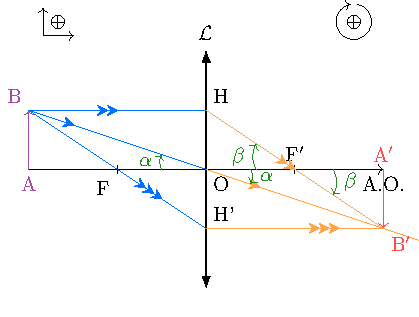
\includegraphics[width=\linewidth, draft=true]{lent_conv-demo}
			}{%
				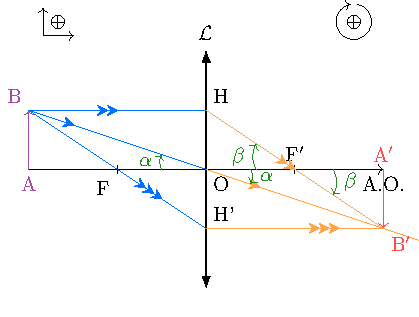
\includegraphics[width=\linewidth]{lent_conv-demo}
			}%
			\captionof{figure}{Schéma \protect \pt{1} \psw{+} \protect \pt{1}}
			\label{fig:lent_rc}
		\end{center}
	\end{isd}

	\item[n]{9} %
	Quelles sont les valeurs maximale et minimale de la focale du cristallin pour
	un œil emmétrope~? On rappelle que la distance cristallin-rétine est $d
		\approx \SI{22.3}{mm}$. Un schéma est attendu pour la situation
	d'accomodation.
	\begin{isd}[righthand ratio=.3]
		\psw{%
			On a
			\begin{gather*}
				\frac{1}{\OFp} \stm{=} \frac{1}{\OAp} - \frac{1}{\OA}
			\end{gather*}
			Or, $\Ar' = \mathrm{E}$ \pt{1} puisque l'image doit se former sur la
			rétine. De plus, $\OA\ind{remotum} = -\infty$ \pt{1} et $\OA\ind{acco} =
				\SI{-25}{cm}$ \pt{1}. Ainsi, on trouve
			\begin{gather*}
				\xul{\OFp_\mathrm{repos} = \SI{22.3}{mm}} \pt{1}
				\qqet \boxed{
					\OFp\ind{acco} \stm{=} \frac{\obarr{OE}\OA}{\OA - \obarr{OE}}
				}
				\\
				\mathrm{A.N.~:}\enskip
				\xul{
					\OFp\ind{acco} = \SI{21}{mm}
				}
				\hspace{12pt}
				\pt{1}
			\end{gather*}
		}%
		\vspace*{-20pt}
		\tcblower
		\begin{center}
			\sswitch{%
				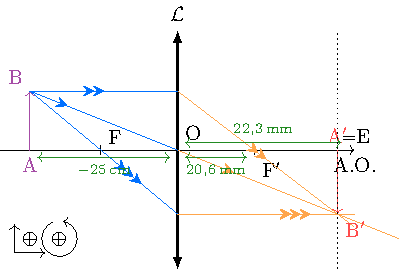
\includegraphics[width=\linewidth, draft=true]{oeil_acco}
			}{%
				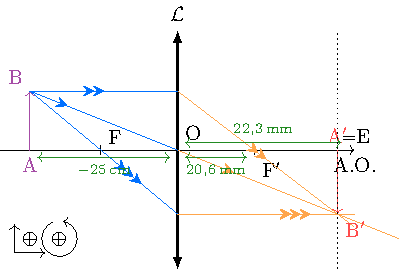
\includegraphics[width=\linewidth]{oeil_acco}
			}%
			\captionof{figure}{Schéma \protect \pt{1} \psw{+} \protect \pt{1}}
		\end{center}
	\end{isd}
	\item[n]{5} %
	Deux lentilles minces convergentes $\Lc_1$ de centre optique O$_1$ et $\Lc_2$
	de centre optique O$_2$ sont disposées selon le schéma ci-dessous. Écrire la
	représentation optique du système, puis trouver la position de l'image finale
	$\ABp$ de l'objet AB donnée par l'association $\Lc_1 + \Lc_2$ par un objet
	intermédiaire, et donner la nature de tous les objets et images.
	\begin{center}
		\sswitch{%
			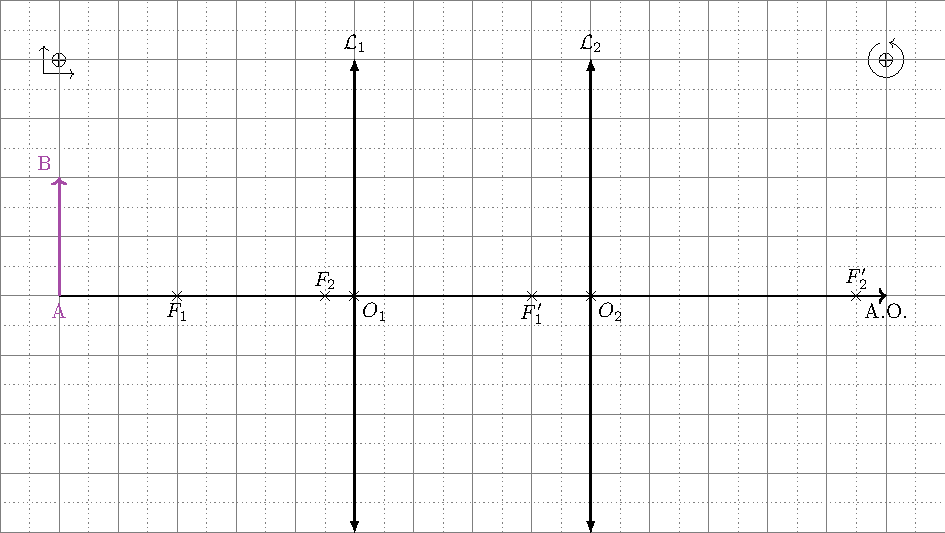
\includegraphics[width=.85\linewidth]{asso_lent-a_plain}
		}{%
			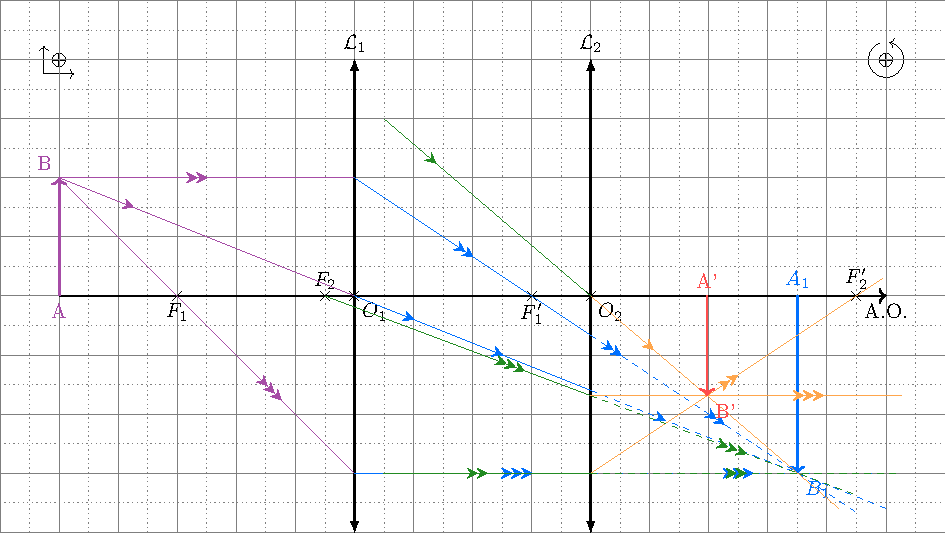
\includegraphics[width=.85\linewidth]{asso_lent-a}
		}%
	\end{center}
	\psw{%
		$\AB \opto{\Lc_1}{O_1} \ABb \opto{\Lc_2}{O_2} \ABp$ \pt{1}. On part d'un
		objet réel pour avoir $\ABb$ \textbf{image réelle pour $\Lc_1$} \pt{1} mais
		\textbf{objet virtuel pour $\Lc_2$}, et finalement $\ABp$ image réelle.
	}%
\end{enumerate}

\vspace{-30pt}
\ifstudent{
	\begin{tikzpicture}[remember picture, overlay]
		\node[anchor=north west, align=left]
		at ([shift={(1.4cm,0)}]current page.north west)
		{\\[5pt]\Large\bfseries Nom~:\\[10pt]\Large\bfseries Prénom~:};
		\node[anchor=north east, align=right]
		at ([shift={(-1.5cm,-17pt)}]current page.north east)
		{\Large\bfseries Note~:\hspace{1cm}/20};
	\end{tikzpicture}
}
\end{document}
